\chapter{Second Derivatives and the Laplacian}
\label{ch:lesson13}

Chapter~\ref{ch:lesson12} found edges as \emph{peaks} in the first derivative (gradient magnitude). This chapter uses the \textbf{second} derivative instead, where edges show up as \textbf{zero crossings} --- the basis of the classic Marr-Hildreth edge detector. We then reuse the same blur-and-difference idea to build a \textbf{Laplacian pyramid}, which fixes the information-loss problem from Chapter~\ref{ch:lesson11}'s Gaussian pyramid.

\section{Why zero crossings? A 1D intuition}

Consider a single step edge along one row. The first derivative is a spike at the edge; the second derivative swings from positive to negative (or vice versa) and crosses exactly zero right at the edge location, as shown in Figure~\ref{fig:l13-1}.

\begin{figure}[h]
\centering
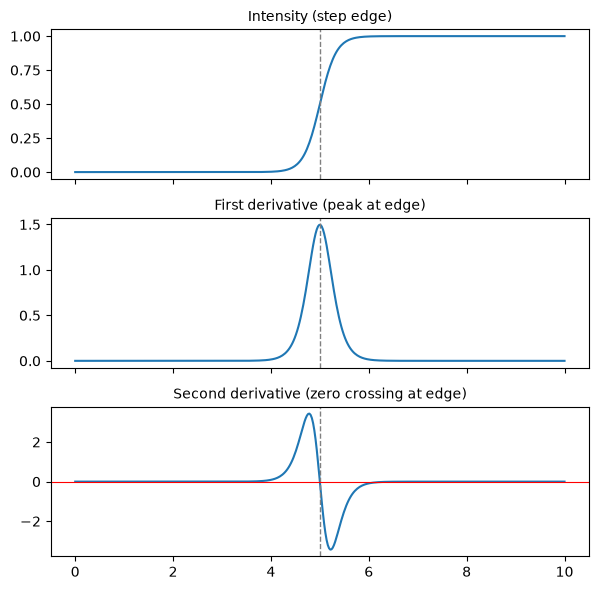
\includegraphics[width=0.5\textwidth]{figures/lesson13_fig01.png}
\caption{A smoothed step edge, its first derivative (a peak), and its second derivative (a zero crossing), all at the same location.}
\label{fig:l13-1}
\end{figure}

\section{The Laplacian: a 2D second derivative}

The Laplacian sums the unmixed second partial derivatives of a 2D image:
\begin{equation}
\nabla^2 I = \frac{\partial^2 I}{\partial x^2} + \frac{\partial^2 I}{\partial y^2}.
\end{equation}
Unlike the gradient, it's a single scalar at each pixel (no direction) --- it just measures how much a pixel differs from the average of its neighbors. Two common discrete kernels:
\begin{equation}
K_4 = \begin{bmatrix}0&1&0\\1&-4&1\\0&1&0\end{bmatrix} \qquad K_8 = \begin{bmatrix}1&1&1\\1&-8&1\\1&1&1\end{bmatrix}.
\end{equation}
$K_4$ uses only the 4-connected neighbors; $K_8$ also includes the diagonals for a stronger, more isotropic response. Convolving with $K_4$ matches \code{cv2.Laplacian(img, cv2.CV\_64F, ksize=1)} exactly, shown in Figure~\ref{fig:laplacian-response}.

\begin{figure}[h]
\centering
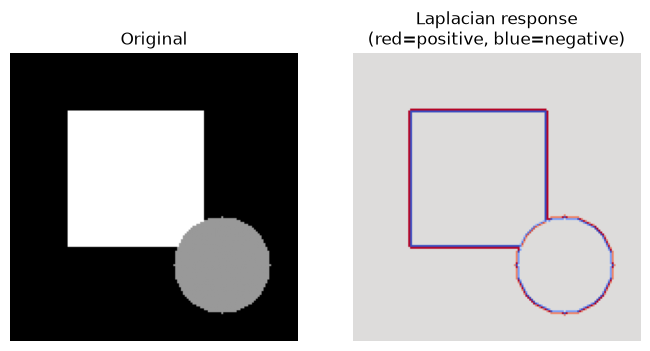
\includegraphics[width=0.6\textwidth]{figures/lesson13_fig02.png}
\caption{Every edge produces a positive lobe on one side and a negative lobe on the other --- the edge itself sits at the zero crossing between them. The response is shown on a red-blue diverging color scale specifically because the Laplacian is signed --- red marks positive values, blue marks negative, making the sign flip at each zero crossing easy to see at a glance.}
\label{fig:laplacian-response}
\end{figure}

\section{The Marr-Hildreth detector: Laplacian of Gaussian (LoG)}

The Laplacian, like any derivative, amplifies high-frequency noise --- and a \emph{second} derivative amplifies it even more than a first derivative does. Marr and Hildreth's fix (\citelink{marrhildreth1980}{Marr \& Hildreth, 1980}): \textbf{smooth first}, then take the Laplacian. Since convolution is associative, this is equivalent to convolving directly with a single combined kernel, the \textbf{Laplacian of Gaussian (LoG)}:
\begin{equation}
\text{LoG}_\sigma(I) = \nabla^2(G_\sigma * I) = (\nabla^2 G_\sigma) * I.
\end{equation}
Edges are then found as \textbf{zero crossings} of the LoG response, rather than by thresholding its magnitude directly, as in Figure~\ref{fig:l13-3}.

\begin{figure}[h]
\centering
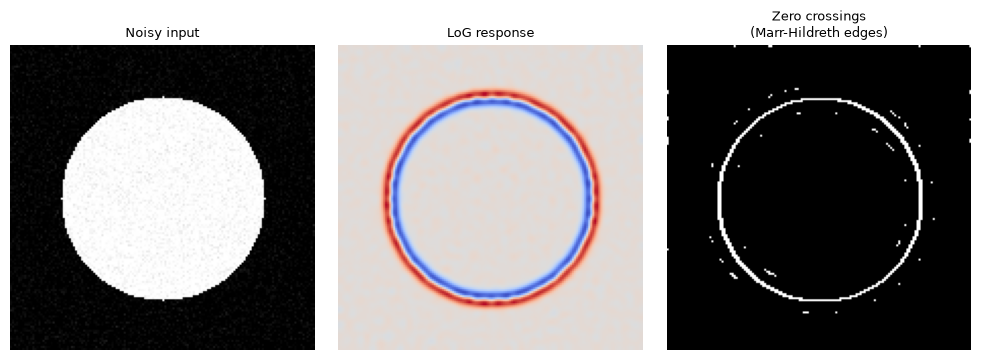
\includegraphics[width=0.9\textwidth]{figures/lesson13_fig03.png}
\caption{A noisy disk, its LoG response, and the resulting zero-crossing edge map (Marr-Hildreth edges). The LoG response uses the same red/blue diverging scale as Figure~\ref{fig:laplacian-response}, for the same reason.}
\label{fig:l13-3}
\end{figure}

\subsection*{The cheaper approximation: Difference of Gaussians (DoG)}

Computing a true LoG kernel is more expensive than blurring. A widely used shortcut: the \emph{difference} of two Gaussian blurs at slightly different scales approximates a scaled LoG:
\begin{equation}
\text{DoG} = G_{\sigma} - G_{k\sigma} \;\approx\; -(k-1)\sigma^2 \cdot \text{LoG}_\sigma.
\end{equation}
This is the same building block later reused by SIFT for keypoint detection at multiple scales. On a test image, the correlation between the true LoG and the scaled DoG comes to $0.967$ --- highly correlated but not identical, since DoG is an approximation, not an exact substitute; a much cheaper one, though (two blurs and a subtraction vs.\ an explicit second-derivative kernel). Figure~\ref{fig:l13-4} shows the two side by side.

\begin{figure}[h]
\centering
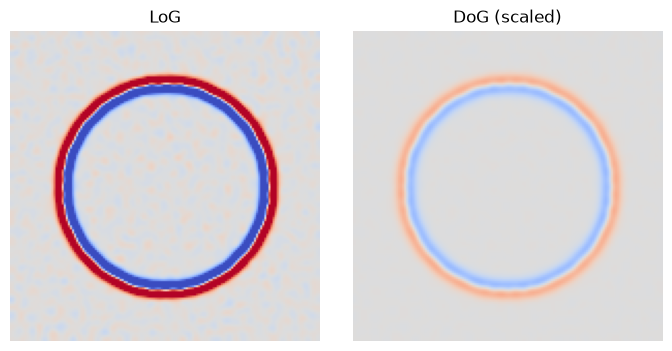
\includegraphics[width=0.6\textwidth]{figures/lesson13_fig04.png}
\caption{LoG response vs.\ the scaled DoG approximation --- visually almost indistinguishable.}
\label{fig:l13-4}
\end{figure}

\section{Laplacian pyramids: recovering what Gaussian pyramids throw away}

Chapter~\ref{ch:lesson11} showed that a Gaussian pyramid loses information: blurring and downsampling repeatedly, then trying to upsample back, doesn't reconstruct the original. A \textbf{Laplacian pyramid} fixes this by storing, at each level, exactly the detail that would otherwise be lost --- the \emph{difference} between a Gaussian level and the coarser level upsampled back to match it. That difference is a discrete approximation of the Laplacian, which is why it shares the name.

\begin{lstlisting}
def laplacian_pyramid(gauss_pyramid):
    lap_pyramid = []
    for i in range(len(gauss_pyramid) - 1):
        size = (gauss_pyramid[i].shape[1], gauss_pyramid[i].shape[0])
        upsampled = cv2.pyrUp(gauss_pyramid[i + 1], dstsize=size)
        detail = gauss_pyramid[i].astype(np.int16) - upsampled.astype(np.int16)
        lap_pyramid.append(detail)
    lap_pyramid.append(gauss_pyramid[-1].astype(np.int16))  # smallest level: no finer detail to subtract
    return lap_pyramid
\end{lstlisting}

Figure~\ref{fig:l13-5} shows the resulting pyramid.

\begin{figure}[h]
\centering
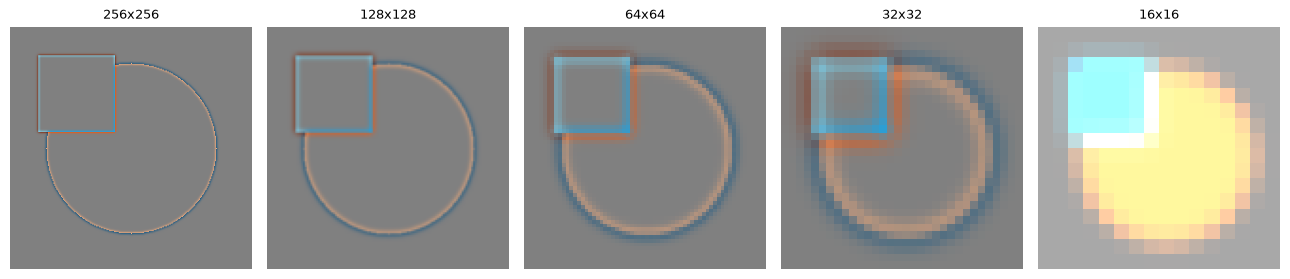
\includegraphics[width=0.95\textwidth]{figures/lesson13_fig05.png}
\caption{A 5-level Laplacian pyramid, each level shifted by $+128$ gray levels so negative values are visible. Each level is mostly flat gray except right at edges --- exactly where detail is lost by blurring and downsampling. The final, smallest level stores actual image content rather than a difference, since there's nothing coarser left to compare it to.}
\label{fig:l13-5}
\end{figure}

\subsection*{Exact reconstruction}

Because each level stores exactly what its Gaussian-pyramid counterpart discarded, summing back up the pyramid reconstructs the original image exactly (up to integer rounding): max reconstruction error is $0$ gray levels, mean error $0.0000$ (Figure~\ref{fig:l13-6}).

\begin{figure}[h]
\centering
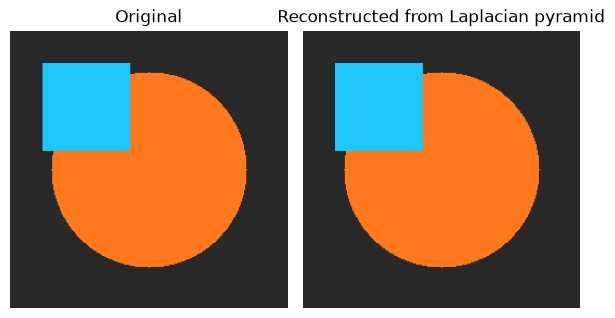
\includegraphics[width=0.55\textwidth]{figures/lesson13_fig06.png}
\caption{Original vs.\ reconstructed-from-Laplacian-pyramid --- pixel-perfect.}
\label{fig:l13-6}
\end{figure}

Compare this to Chapter~\ref{ch:lesson11}'s \code{pyrDown} + \code{pyrUp} result, which had a visibly nonzero reconstruction error: the Laplacian pyramid stores just enough extra information at each level to make the process perfectly reversible, at the cost of needing to keep all the levels around (not just the smallest one).

\subsection*{Exercises}
\begin{enumerate}
  \item Try \code{threshold=1.0} and \code{threshold=15.0} in \code{zero\_crossings}. How does the number of detected edge pixels change, and why does a \emph{higher} threshold on a \emph{second}-derivative sign-change criterion behave differently than a magnitude threshold on a first derivative?
  \item Increase the noise level in the noisy disk and see how large \code{sigma} needs to be before the zero-crossing edge map stops being dominated by spurious noise loops.
  \item Laplacian pyramids are the classic tool behind seamless image blending (e.g.\ blending two photos along a mask, level by level). Sketch out --- in words or code --- how you'd blend two Laplacian pyramids before reconstructing, and why blending in this representation avoids sharp seams that blending the original images directly would produce.
\end{enumerate}

\vfill
\fullcode{lesson13}{lesson13_laplacian_pyramids}
